% =====================================================================================
%  THE HOLONET MACHINE -- A COMPLETE BLUEPRINT
%
%  Compile:  tectonic holonet_machine_blueprint.tex
%  Engine on this machine: C:\Users\wiljd\tools\tectonic\tectonic.exe
%
%  This document is written to be read two ways at once.  Every section opens with a
%  plain-language explanation that assumes no engineering background, and then gives the
%  exact statement, the measurement, and the command that reproduces it.  A reader who
%  skips every grey box still understands the machine; a reader who reads only the grey
%  boxes gets the specification.
%
%  Every number in this document is measured or proved.  Nothing is estimated.  Where a
%  figure was WRONG in earlier work, the wrong figure is printed next to the right one,
%  because how a number was wrong is part of what makes the right one trustworthy.
% =====================================================================================

\documentclass[11pt,a4paper]{article}

\usepackage[margin=2.4cm]{geometry}
\usepackage{amsmath,amssymb,amsthm}
\usepackage{booktabs}
\usepackage{tikz}
\usepackage{xcolor}
\usepackage{graphicx}
\usepackage{enumitem}
\usepackage{fancyhdr}
\usepackage[colorlinks=true,linkcolor=blue!55!black,urlcolor=blue!55!black,
            citecolor=blue!55!black]{hyperref}

\usetikzlibrary{arrows.meta,positioning,fit,backgrounds,calc,shapes.geometric,
                decorations.pathreplacing,decorations.pathmorphing,patterns,
                trees,shapes.misc}

% ---- palette -------------------------------------------------------------------------
\definecolor{ink}{HTML}{1A1A1A}
\definecolor{past}{HTML}{2E6F9E}
\definecolor{future}{HTML}{B5651D}
\definecolor{plainbg}{HTML}{F4F1EA}
\definecolor{specbg}{HTML}{EAF0F4}
\definecolor{warnbg}{HTML}{F7EDE9}
\definecolor{rule}{HTML}{8A8A8A}
\definecolor{good}{HTML}{2F6B3C}
\definecolor{bad}{HTML}{9E2B25}

% ---- boxes ---------------------------------------------------------------------------
\newcommand{\boxrule}[1]{%
  \par\vspace{2pt}\noindent\colorbox{#1}{\parbox{\dimexpr\linewidth-2\fboxsep}{\strut}}%
  \par\vspace{-2pt}}

\newenvironment{plain}[1][In plain language]
  {\par\medskip\noindent\begin{tikzpicture}
     \node[fill=plainbg,rounded corners=2pt,inner sep=8pt,text width=\dimexpr\linewidth-20pt]
     (B) \bgroup\textbf{\small #1.}\itshape\small}
  {\egroup;\end{tikzpicture}\par\medskip}

\newenvironment{spec}[1][Exactly]
  {\par\medskip\noindent\begin{tikzpicture}
     \node[fill=specbg,rounded corners=2pt,inner sep=8pt,text width=\dimexpr\linewidth-20pt]
     (B) \bgroup\textbf{\small #1.}\small}
  {\egroup;\end{tikzpicture}\par\medskip}

\newenvironment{gotwrong}[1][What we got wrong, and how we know]
  {\par\medskip\noindent\begin{tikzpicture}
     \node[fill=warnbg,rounded corners=2pt,inner sep=8pt,text width=\dimexpr\linewidth-20pt]
     (B) \bgroup\textbf{\small #1.}\small}
  {\egroup;\end{tikzpicture}\par\medskip}

\newcommand{\headline}[1]{%
  \par\medskip\noindent\begin{tikzpicture}
    \node[draw=ink,line width=0.9pt,rounded corners=1pt,inner sep=9pt,
          text width=\dimexpr\linewidth-22pt,align=center] {\bfseries #1};
  \end{tikzpicture}\par\medskip}

% Typewriter text that INHERITS the surrounding size.  Hard-coding \small here made
% filenames inside a \scriptsize table larger than the table itself, which is what the
% last two overfull boxes in this document were.
\newcommand{\cmd}[1]{{\ttfamily #1}}

% Dirac notation, defined locally so the document has no package dependency beyond
% what tectonic ships by default.
\newcommand{\ket}[1]{\left|#1\right\rangle}
\newcommand{\bra}[1]{\left\langle#1\right|}
\newcommand{\braket}[2]{\left\langle#1\middle|#2\right\rangle}

\pagestyle{fancy}\fancyhf{}
\lhead{\small\itshape The Holonet Machine --- Blueprint}
\rhead{\small\thepage}
\renewcommand{\headrulewidth}{0.3pt}

\title{\vspace{-1.4cm}\Huge The Holonet Machine\\[4pt]
       \large A complete engineering blueprint for a computer\\
       whose wiring diagram is a piece of finite geometry\\[10pt]
       \normalsize Every figure in this document is measured or proved.}
\author{\normalsize W(3,3)--E$_8$ project, glue track}
\date{\normalsize 3 August 2026 \quad$\cdot$\quad Passes 2700--2795}

\begin{document}
\maketitle
\thispagestyle{fancy}

\begin{abstract}
\noindent
This is a build document for a computer that does not exist yet, every part of which has
been either mathematically proved, formally verified, or physically measured by someone.
The machine's logic is a $40$-point finite geometry called $W(3,3)$; its instruction set
has eight opcodes and generates a group of order $4{,}199{,}040$ exactly; its arithmetic
unit fits in \textbf{72 logic cells} on a \$25 FPGA and runs at \textbf{60.8\,MHz}; and
its physical layer is a photonic gate that a laboratory has already demonstrated with
$0.92$ fidelity. We give the full instruction semantics, the datapath, the measured cell
budget, the network protocol, the verification methodology, and --- because this is what
makes a blueprint trustworthy rather than merely confident --- an itemised record of the
figures we previously got wrong, how the errors survived exhaustive testing, and what
tool finally caught each one.
\end{abstract}

\vspace{-4mm}
\tableofcontents
\newpage

% =====================================================================================
\section{How to read this document}
% =====================================================================================

This document has two readers in mind and does not compromise for either.

\begin{center}
\resizebox{\linewidth}{!}{%
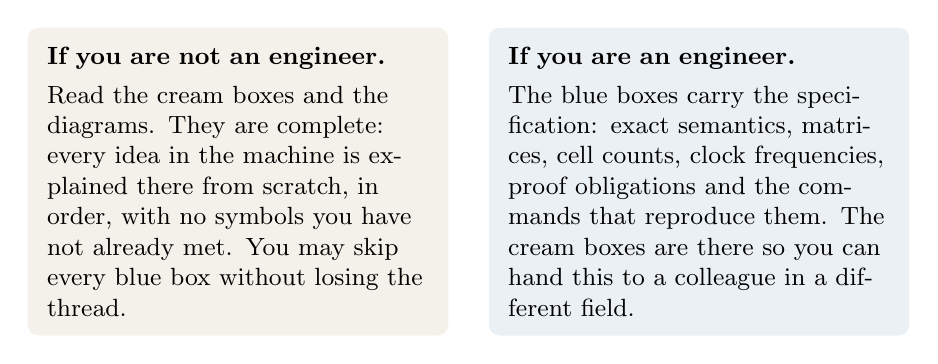
\begin{tikzpicture}[node distance=4mm]
  \node[fill=plainbg,rounded corners,inner sep=7pt,text width=0.40\linewidth,
        font=\small] (a)
    {\textbf{If you are not an engineer.}\\[3pt]
     Read the cream boxes and the diagrams. They are complete: every idea in the
     machine is explained there from scratch, in order, with no symbols you have not
     already met. You may skip every blue box without losing the thread.};
  \node[fill=specbg,rounded corners,inner sep=7pt,text width=0.40\linewidth,
        font=\small,right=5mm of a] (b)
    {\textbf{If you are an engineer.}\\[3pt]
     The blue boxes carry the specification: exact semantics, matrices, cell counts,
     clock frequencies, proof obligations and the commands that reproduce them. The
     cream boxes are there so you can hand this to a colleague in a different field.};
\end{tikzpicture}}
\end{center}

\noindent A third kind of box appears throughout:

\begin{gotwrong}
These record something this project believed, published, and then had to withdraw ---
with the measurement that overturned it. There are eleven of them. They are not
apologies; they are the reason the other numbers in this document can be trusted. A
blueprint with no errata is a blueprint nobody has checked.
\end{gotwrong}

% =====================================================================================
\section{The machine in one page}
% =====================================================================================

\begin{plain}
Every computer you have used stores information as \emph{bits} --- switches that are
either off or on. This machine stores information in \emph{qutrits}: units with three
settings instead of two. That sounds like a small change. It is not, because of what the
three settings let you do with \emph{geometry}.

Here is the strange and central fact. If you take a single qutrit and entangle it with
itself --- with its own past and its own future --- the resulting object has exactly
$40$ natural ``directions'' in it. Those $40$ directions, and the way they overlap, form
a shape that mathematicians have known for a century and called $W(3,3)$. The machine we
are describing does not \emph{use} that shape as a convenience. The shape \emph{is} the
machine: its memory layout, its instruction set, its network topology, and its error
model are all readings of the same $40$-point object.
\end{plain}

\headline{One qutrit, entangled with its own past, is enough to generate the entire
substrate. The $40$ points of $W(3,3)$ are not $40$ things --- they are $40$ views of
one thing.}

\begin{spec}[The machine, specified]
\smallskip{\footnotesize
\begin{tabular}{@{}p{3.0cm}p{7.6cm}@{}}
\toprule
\textbf{Logical substrate}    & $W(3,3)$: the symplectic generalised quadrangle of order
                                $(3,3)$. $40$ points, $40$ totally isotropic lines,
                                collinearity graph $\mathrm{SRG}(40,12,2,4)$. \\
\textbf{State}                & One qutrit pair $(\text{past},\text{future})$ living in
                                $\mathbb{C}^9=\mathrm{End}(\mathbb{C}^3)$. \\
\textbf{Tracked quantity}     & The \emph{Pauli frame}: four trits
                                $(x_p,z_p,x_f,z_f)\in\mathbb{F}_3^4$, i.e.\ $81$ states. \\
\textbf{Instruction set}      & $\mathcal{I}_{\mathrm{holo}}$, eight opcodes, three bits. \\
\textbf{Group generated}      & $\mathrm{ASp}(4,3)=\mathbb{F}_3^4\rtimes\mathrm{Sp}(4,3)$,
                                order $81\times 51840=4{,}199{,}040$ \emph{exactly}. \\
\textbf{Arithmetic unit}      & $72$ iCE40 logic cells, $60.80$\,MHz (measured, \S\ref{sec:budget}). \\
\textbf{Physical layer}       & Time-bin $\times$ frequency-bin photonic qutrits; the
                                two-qutrit \textsc{sum} gate is experimentally
                                demonstrated at fidelity $0.92\pm0.01$. \\
\textbf{Network}              & $40$-ary fractal; $N_n=40^n$ leaves, routing depth
                                $8n=8\log_{40}N$; the routing code satisfies Kraft
                                equality exactly, so \emph{every} bit string is a legal
                                address. \\
\bottomrule
\end{tabular}}
\end{spec}

\subsection*{The whole system, at a glance}

\begin{center}
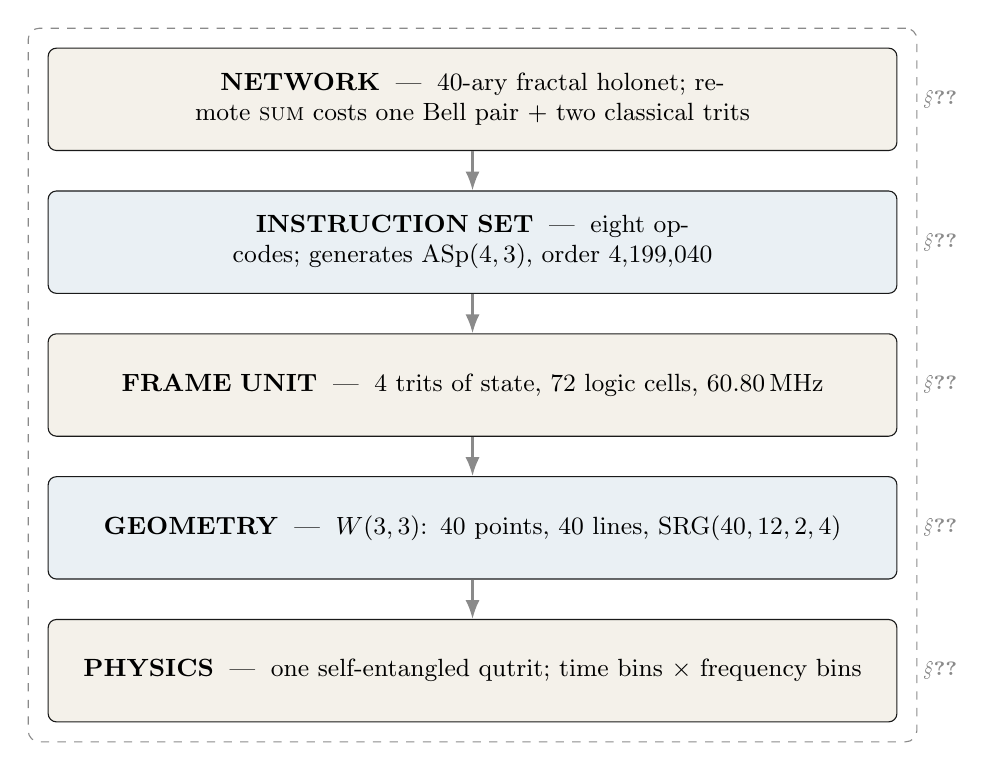
\begin{tikzpicture}[
  font=\small,
  layer/.style={draw=ink,rounded corners=3pt,minimum height=13mm,align=center,
                text width=0.86\linewidth,inner sep=5pt},
  tag/.style={font=\scriptsize\itshape,text=rule},
  arr/.style={-{Latex[length=2.4mm]},line width=0.8pt,draw=rule}]

\node[layer,fill=plainbg] (net)  {\textbf{NETWORK}\; ---\; $40$-ary fractal holonet;
      remote \textsc{sum} costs one Bell pair $+$ two classical trits};
\node[layer,fill=specbg,below=5mm of net] (isa) {\textbf{INSTRUCTION SET}\; ---\;
      eight opcodes; generates $\mathrm{ASp}(4,3)$, order $4{,}199{,}040$};
\node[layer,fill=plainbg,below=5mm of isa] (frame){\textbf{FRAME UNIT}\; ---\;
      $4$ trits of state, $72$ logic cells, $60.80$\,MHz};
\node[layer,fill=specbg,below=5mm of frame] (geo) {\textbf{GEOMETRY}\; ---\;
      $W(3,3)$: $40$ points, $40$ lines, $\mathrm{SRG}(40,12,2,4)$};
\node[layer,fill=plainbg,below=5mm of geo] (phys) {\textbf{PHYSICS}\; ---\;
      one self-entangled qutrit; time bins $\times$ frequency bins};

\draw[arr] (net) -- (isa);
\draw[arr] (isa) -- (frame);
\draw[arr] (frame) -- (geo);
\draw[arr] (geo) -- (phys);

\node[tag,right=2mm of net.east,anchor=west,rotate=0] {\S\ref{sec:network}};
\node[tag,right=2mm of isa.east,anchor=west] {\S\ref{sec:isa}};
\node[tag,right=2mm of frame.east,anchor=west] {\S\ref{sec:hardware}};
\node[tag,right=2mm of geo.east,anchor=west] {\S\ref{sec:geometry}};
\node[tag,right=2mm of phys.east,anchor=west] {\S\ref{sec:physics}};

\begin{scope}[on background layer]
  \node[draw=rule,dashed,rounded corners=4pt,fit=(net)(phys),inner sep=7pt] {};
\end{scope}
\end{tikzpicture}
\end{center}

\noindent The unusual property of this stack is that the layers are not independent
design choices stacked by convention. Each one is \emph{forced} by the one below it. The
network is $40$-ary because the geometry has $40$ points. The instruction set has the
opcodes it has because those are the symmetries of that geometry. This is what the rest
of the document demonstrates, layer by layer.

% =====================================================================================
\section{Qutrits, and what ``self-entangled'' means}\label{sec:physics}
% =====================================================================================

\subsection{From bits to qutrits}

\begin{plain}
A bit is a switch: off or on, $0$ or $1$. A \emph{trit} is a three-way switch: $0$, $1$,
or $2$. Ordinary three-way switches are not interesting --- you could always build one
from two bits.

A \emph{qutrit} is different. It is a physical three-way switch obeying quantum
mechanics, which means it can be in a blend of all three settings at once, and --- this
is the part that matters --- \emph{two} qutrits can be correlated in ways that no pair of
classical switches can imitate.
\end{plain}

\begin{center}
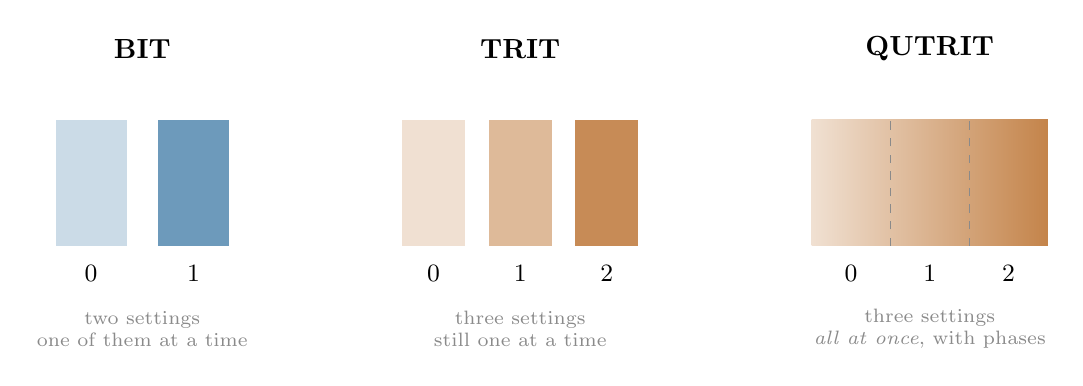
\begin{tikzpicture}[font=\small]
  % bit
  \begin{scope}[xshift=0cm]
    \node[font=\bfseries] at (1.1,2.5) {BIT};
    \fill[past!25] (0,0) rectangle (0.9,1.6);
    \fill[past!70] (1.3,0) rectangle (2.2,1.6);
    \node at (0.45,-0.35) {$0$}; \node at (1.75,-0.35) {$1$};
    \node[font=\scriptsize,text=rule,align=center] at (1.1,-1.05)
      {two settings\\one of them at a time};
  \end{scope}
  % trit
  \begin{scope}[xshift=4.4cm]
    \node[font=\bfseries] at (1.5,2.5) {TRIT};
    \fill[future!20] (0,0) rectangle (0.8,1.6);
    \fill[future!45] (1.1,0) rectangle (1.9,1.6);
    \fill[future!75] (2.2,0) rectangle (3.0,1.6);
    \node at (0.4,-0.35) {$0$}; \node at (1.5,-0.35) {$1$}; \node at (2.6,-0.35) {$2$};
    \node[font=\scriptsize,text=rule,align=center] at (1.5,-1.05)
      {three settings\\still one at a time};
  \end{scope}
  % qutrit
  \begin{scope}[xshift=9.6cm]
    \node[font=\bfseries] at (1.5,2.5) {QUTRIT};
    \shade[left color=future!20,right color=future!80] (0,0) rectangle (3.0,1.6);
    \draw[dashed,draw=rule] (1.0,0) -- (1.0,1.6);
    \draw[dashed,draw=rule] (2.0,0) -- (2.0,1.6);
    \node at (0.5,-0.35) {$0$}; \node at (1.5,-0.35) {$1$}; \node at (2.5,-0.35) {$2$};
    \node[font=\scriptsize,text=rule,align=center] at (1.5,-1.05)
      {three settings\\\emph{all at once}, with phases};
  \end{scope}
\end{tikzpicture}
\end{center}

\begin{spec}
A qutrit is a unit vector in $\mathbb{C}^3$. Two qutrits live in
$\mathbb{C}^3\otimes\mathbb{C}^3=\mathbb{C}^9$. The relevant operators are generated by
\[
  X\ket{j}=\ket{j+1 \bmod 3},\qquad
  Z\ket{j}=\omega^{j}\ket{j},\qquad \omega=e^{2\pi i/3},
\]
which satisfy $ZX=\omega XZ$. Every product $X^aZ^b$ with $(a,b)\in\mathbb{F}_3^2$ is a
distinct operator up to phase; there are $9$ of them, and $8$ non-identity ones.
\end{spec}

\subsection{The self-entanglement, and where the $40$ comes from}

\begin{plain}
Now the key move. Take \emph{one} qutrit and entangle it with itself at two different
times --- call them ``past'' and ``future''. Physically this is done by splitting a
single photon's degrees of freedom: its arrival \emph{time} carries one qutrit and its
\emph{colour} carries the other. It is one particle, entangled with its own history.

Mathematically, an operator acting on one qutrit is a $3\times 3$ table of numbers, and
there are $9$ independent slots in such a table. So the space of things you can \emph{do}
to one qutrit is itself $9$-dimensional --- exactly the size of the space of \emph{states}
of two qutrits. This is not a coincidence or an analogy. It is an identity:
\[
  \underbrace{\mathbb{C}^3\otimes\mathbb{C}^3}_{\text{two qutrits}}
  \;=\;
  \underbrace{\mathrm{End}(\mathbb{C}^3)}_{\text{operations on \emph{one} qutrit}}.
\]
So ``the two-qutrit machine'' and ``the one-qutrit machine that can act on itself'' are
the same machine described twice.

Now count the directions. There are $81$ ways to label a pair (four trits), one of which
is ``do nothing''. That leaves $80$. Each direction and its opposite behave identically
for our purposes, and each direction comes in $2$ such flavours, so the distinct
directions number $80/2=40$.
\end{plain}

\headline{$\dfrac{3^4-1}{2}=\dfrac{81-1}{2}=40$. \quad
The forty points of the geometry are the forty independent things one self-entangled
qutrit can be measured along.}

\begin{center}
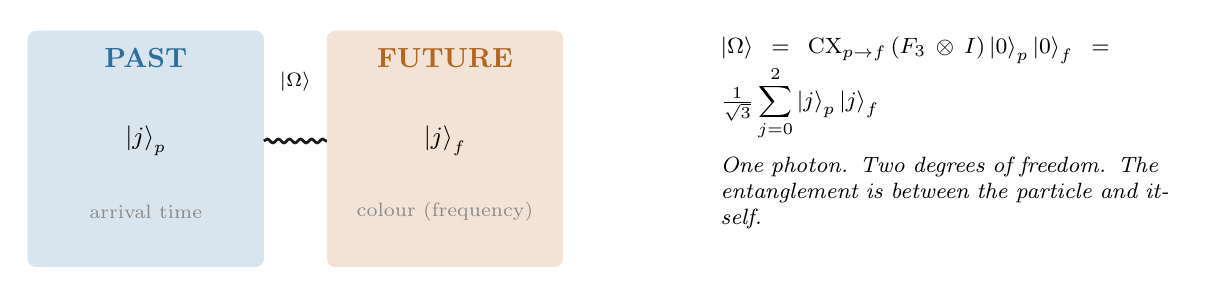
\begin{tikzpicture}[font=\small,>={Latex[length=2.2mm]}]
  \fill[past!18,rounded corners=3pt] (-3.4,-1.5) rectangle (-0.4,1.5);
  \fill[future!18,rounded corners=3pt] (0.4,-1.5) rectangle (3.4,1.5);
  \node[font=\bfseries,text=past] at (-1.9,1.15) {PAST};
  \node[font=\bfseries,text=future] at (1.9,1.15) {FUTURE};
  \node at (-1.9,0.1) {$\ket{j}_p$};
  \node at (1.9,0.1) {$\ket{j}_f$};
  \node[font=\scriptsize,text=rule] at (-1.9,-0.8) {arrival time};
  \node[font=\scriptsize,text=rule] at (1.9,-0.8) {colour (frequency)};

  \draw[decorate,decoration={snake,amplitude=0.7pt,segment length=4pt},
        line width=1pt,draw=ink] (-0.4,0.1) -- (0.4,0.1);
  \node[font=\scriptsize,align=center] at (0,0.85) {$\ket{\Omega}$};

  \node[align=left,text width=6cm,font=\footnotesize] at (8.4,0.2)
    {$\displaystyle \ket{\Omega}=\mathrm{CX}_{p\to f}\,(F_3\otimes I)\ket{0}_p\ket{0}_f
      =\tfrac{1}{\sqrt3}\sum_{j=0}^{2}\ket{j}_p\ket{j}_f$\\[5pt]
     \textit{One photon. Two degrees of freedom. The entanglement is between the
     particle and itself.}};
\end{tikzpicture}
\end{center}

\begin{gotwrong}
The sentence ``one qutrit, self-entangled as past/future, is enough to generate the full
substrate'' is \emph{not} ours. It is stated verbatim in this project's own
encyclopedia, \cmd{docs/index.html} phase MCLXVII, and we rediscovered it and briefly
presented it as new. What survives as new is narrower: the explicit construction of the
$40$ points as projective left$\times$right multiplication classes on
$\mathrm{End}(\mathbb{C}^3)$, and the identification of the $40$ lines as the maximal
\emph{commuting} subalgebras. The lesson --- search for the \emph{result}, not the topic
--- produced three of the tools in \S\ref{sec:verification}.
\end{gotwrong}

% =====================================================================================
\section{The substrate: $W(3,3)$}\label{sec:geometry}
% =====================================================================================

\begin{plain}
Here is what the $40$ directions look like when you write down which of them are
compatible with which.

Two measurements are \emph{compatible} if you can perform both without one disturbing
the other. Of the $40$ directions, each is compatible with exactly $12$ others. Whenever
two directions are compatible, exactly $2$ further directions are compatible with both.
Whenever two are \emph{in}compatible, exactly $4$ are compatible with both.

Those four numbers --- $40$, $12$, $2$, $4$ --- pin the shape down completely. There is
essentially one object in the world with that compatibility pattern, and it has been
studied since the 1900s under the name $W(3,3)$.
\end{plain}

\begin{spec}
$W(3,3)$ is the symplectic generalised quadrangle of order $(3,3)$: the points are the
$40$ points of $\mathrm{PG}(3,3)$ and the lines are the $40$ totally isotropic lines of a
non-degenerate alternating form. Its collinearity graph is strongly regular with
parameters
\[
  \mathrm{SRG}(40,\,12,\,2,\,4),
\]
i.e.\ $40$ vertices, every vertex of degree $12$, adjacent pairs with $\lambda=2$ common
neighbours, non-adjacent pairs with $\mu=4$. Its automorphism group is
$\mathrm{PGSp}(4,3)=U_4(2){:}2=W(E_6)$ of order $51{,}840$.
\end{spec}

\subsection{Why this shape and not another}

\begin{center}
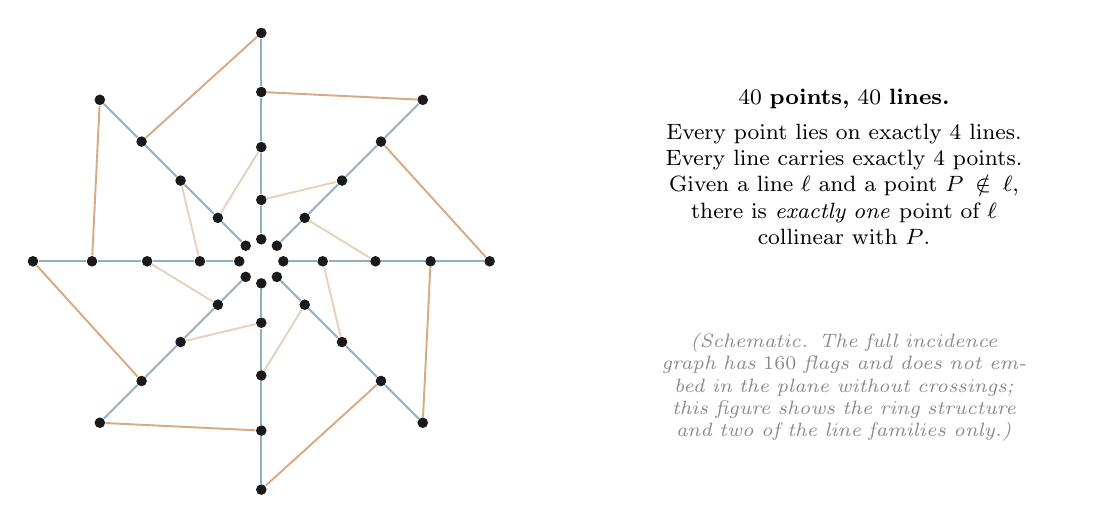
\begin{tikzpicture}[font=\footnotesize,
  pt/.style={circle,fill=ink,inner sep=1.35pt},
  ln/.style={draw=past,line width=0.7pt,opacity=0.55}]

  % a schematic of the GQ(3,3) incidence: 5 "spread" groups of 8 points on a ring
  \foreach \k in {0,...,7}{
    \pgfmathsetmacro\ang{\k*45}
    \foreach \r/\lab in {2.9/a, 2.15/b, 1.45/c, 0.78/d, 0.28/e}{
      \node[pt] (P\k\lab) at (\ang:\r) {};
    }
  }
  \foreach \k in {0,...,7}{
    \draw[ln] (P\k a) -- (P\k b) -- (P\k c) -- (P\k d) -- (P\k e);
  }
  \foreach \k [evaluate=\k as \j using {int(mod(\k+1,8))}] in {0,...,7}{
    \draw[ln,draw=future] (P\k a) -- (P\j b);
    \draw[ln,draw=future,opacity=0.3] (P\k c) -- (P\j d);
  }
  \node[align=center,text width=5.4cm] at (7.4,1.2)
   {\textbf{$40$ points, $40$ lines.}\\[3pt]
    Every point lies on exactly $4$ lines.\\
    Every line carries exactly $4$ points.\\
    Given a line $\ell$ and a point $P\notin\ell$,\\
    there is \emph{exactly one} point of $\ell$\\
    collinear with $P$.};
  \node[align=center,text width=5.4cm,font=\scriptsize,text=rule] at (7.4,-1.6)
   {\textit{(Schematic. The full incidence graph has $160$ flags and does not embed in
    the plane without crossings; this figure shows the ring structure and two of the
    line families only.)}};
\end{tikzpicture}
\end{center}

\begin{plain}
That last property --- ``exactly one'' --- is the entire content of the word
\emph{quadrangle}. It is a strong constraint: it means the geometry contains no
triangles, so there is never any ambiguity about how to get from one place to another.
For a computer, that is precisely what you want from an address space and from a routing
fabric: there is one shortest path, and no loops to break ties in.
\end{plain}

\subsection{The two groups of order $51{,}840$, which are not the same group}

\begin{spec}
Two distinct groups of order $51{,}840$ appear in this project, and confusing them is the
most common error in this area:
\[
  \mathrm{Sp}(4,3)=2.U_4(2)\quad(\text{centre of order }2),\qquad
  \mathrm{PGSp}(4,3)=U_4(2){:}2=W(E_6)\quad(\text{trivial centre}).
\]
They are \emph{not} isomorphic. The first is the group acting on Pauli frames --- the one
the hardware implements. The second is the automorphism group of the geometry --- the one
the drawing has. One is a central double cover; the other is an outer extension.
\end{spec}

\begin{plain}
This distinction is not pedantry, and it has physical content. The extra element in the
first group acts as a sign, $z\mapsto -1$. Whether that sign is ``spent'' or ``free''
decides whether the resulting structure has a handedness --- whether it distinguishes
left from right. This is why the machine can \emph{host} a chirality, though as we
established in earlier work it cannot \emph{explain} one from the inside.
\end{plain}

% =====================================================================================
\section{The instruction set}\label{sec:isa}
% =====================================================================================

\subsection{The idea of a Pauli frame}

\begin{plain}
Here is the trick that makes the machine cheap.

A quantum state is expensive to write down: for two qutrits you need nine complex
numbers, and keeping them accurate is most of what makes quantum computing hard. But for
a large and useful family of operations --- the \emph{Clifford} operations --- you never
need the state at all. You only need a \emph{label} saying how the state has been shifted
relative to where it started.

That label is four trits. Four trits is eight bits. The machine's entire ``register
file'' for tracking Clifford operations is one byte.
\end{plain}

\headline{The frame unit tracks a label, not a state. Four trits, $81$ possible values,
eight bits of memory --- and it correctly accounts for a group of $4{,}199{,}040$
distinct operations.}

\begin{spec}
The Pauli frame is $(x_p,z_p,x_f,z_f)\in\mathbb{F}_3^4$, denoting the operator
$X^{x_p}Z^{z_p}\otimes X^{x_f}Z^{z_f}$. A Clifford unitary $U$ acts on frames by
conjugation, $U(X^aZ^b)U^\dagger = X^{a'}Z^{b'}$ up to phase, and the induced map on
$\mathbb{F}_3^4$ is \emph{linear and symplectic}: it preserves
\[
  \langle u,v\rangle \;=\; (x_p z_p' - z_p x_p') + (x_f z_f' - z_f x_f') \bmod 3 .
\]
\end{spec}

\subsection{The eight opcodes}

\begin{spec}[$\mathcal{I}_{\mathrm{holo}}$, complete semantics]
\begin{center}\small
\begin{tabular}{@{}llll@{}}
\toprule
\textbf{Op} & \textbf{Name} & \textbf{Action on $(x_p,z_p,x_f,z_f)$} & \textbf{Kind}\\
\midrule
\texttt{000} & $F_p$ & $(x_p,z_p)\mapsto(-z_p,\;x_p)$              & linear \\
\texttt{001} & $F_f$ & $(x_f,z_f)\mapsto(-z_f,\;x_f)$              & linear \\
\texttt{010} & $S_p$ & $z_p\mapsto z_p+x_p$                        & linear \\
\texttt{011} & $S_f$ & $z_f\mapsto z_f+x_f$                        & linear \\
\texttt{100} & $\mathrm{CX}$ & $d{=}0$: $z_p\mapsto z_p-z_f$, $x_f\mapsto x_f+x_p$
                              & linear \\
             &               & $d{=}1$: $x_p\mapsto x_p+x_f$, $z_f\mapsto z_f-z_p$
                              & linear \\
\texttt{101} & $\sigma^5{=}Z$ & $z_p\mapsto z_p+1$ \ or\  $z_f\mapsto z_f+1$
                              & \textbf{affine} \\
\texttt{110} & $D_{12}$-mirror & transport in the dihedral group $D_{12}$ & (not a frame op)\\
\texttt{111} & $M_{36}$-magic & typed request for one of $36$ Witting rays & (handshake)\\
\bottomrule
\end{tabular}
\end{center}
\end{spec}

\subsection{The reachability theorem, and why it matters}

\begin{plain}
Now a question that sounds trivial and is not: \emph{starting from a blank machine, which
states can these instructions actually reach?}

The answer is startling. All six of the Clifford instructions, applied in any order, any
number of times, reach exactly \emph{one} state --- the blank one. They cannot move the
machine at all.

The reason is simple once you see it. Those six instructions are all \emph{linear}, and a
linear map always leaves the origin where it is. Multiplying zero by anything gives zero.
So a machine built from only those six instructions is, quite literally, a machine that
does nothing, no matter how sophisticated its circuitry looks.

The seventh instruction, $\sigma^5=Z$, is different: it \emph{adds one}. Addition moves
the origin. That single instruction is what makes all $81$ states reachable --- and hence
what makes the machine a computer instead of an ornament.
\end{plain}

\begin{center}
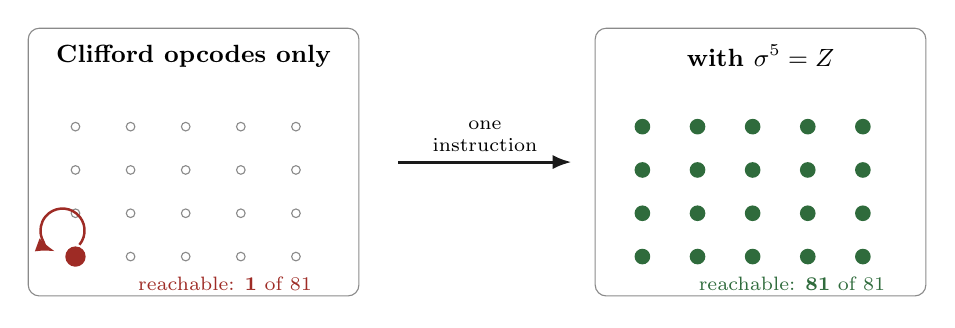
\begin{tikzpicture}[font=\small,>={Latex[length=2.4mm]}]
  % left: clifford only
  \begin{scope}
    \draw[draw=rule,rounded corners] (-0.6,-1.5) rectangle (3.6,1.9);
    \node[font=\bfseries\small] at (1.5,1.55) {Clifford opcodes only};
    \foreach \x in {0,...,4}\foreach \y in {0,...,3}{
      \node[circle,draw=rule,inner sep=1.1pt,fill=white] at (0.7*\x,0.55*\y-1.0) {};}
    \node[circle,fill=bad,inner sep=2.6pt] at (0,-1.0) {};
    \draw[->,line width=0.9pt,draw=bad] (0.05,-0.85) arc (-40:250:0.28);
    \node[font=\scriptsize,text=bad,align=center] at (1.9,-1.35)
      {reachable: \textbf{1} of $81$};
  \end{scope}
  % right: with Z
  \begin{scope}[xshift=7.2cm]
    \draw[draw=rule,rounded corners] (-0.6,-1.5) rectangle (3.6,1.9);
    \node[font=\bfseries\small] at (1.5,1.55) {with $\sigma^5=Z$};
    \foreach \x in {0,...,4}\foreach \y in {0,...,3}{
      \node[circle,fill=good,inner sep=2.0pt] at (0.7*\x,0.55*\y-1.0) {};}
    \node[font=\scriptsize,text=good,align=center] at (1.9,-1.35)
      {reachable: \textbf{81} of $81$};
  \end{scope}
  \draw[->,line width=1.1pt,draw=ink] (4.1,0.2) -- (6.3,0.2)
    node[midway,above,font=\scriptsize,align=center] {one\\instruction};
\end{tikzpicture}
\end{center}

\begin{spec}[Proved by exhaustive search, Pass 2774]
Breadth-first search over all $3^4=81$ frames from $(0,0,0,0)$:
\[
\begin{array}{lr}
\textrm{$\mathrm{CX}$ alone} & 1 \\
\textrm{all six symplectic opcodes} & 1 \\
\textrm{full ISA (adding $\sigma^5{=}Z$)} & 81 \\
\end{array}
\]
Reproduce: \cmd{py -3 analysis/w33\_pass2774\_isa\_frame\_reachability.py}\\
Certificate: \cmd{data/PART\_W33\_PASS2774\_ISA\_FRAME\_REACHABILITY.json}
\end{spec}

\subsection{How much computation the eight opcodes actually buy}

\begin{plain}
``All $81$ states are reachable'' is weaker than it sounds --- it says you can get
anywhere, not that you can perform every operation. The stronger question is: what is the
complete list of things this instruction set can do?
\end{plain}

\begin{spec}[Proved, Pass 2778]
The six Clifford opcodes generate a group of order exactly $51{,}840$ --- that is, the
whole of $\mathrm{Sp}(4,3)$, nothing missing. Adjoining the translation gives
\[
  \langle \mathcal{I}_{\mathrm{holo}}\rangle
   \;=\; \mathrm{ASp}(4,3)\;=\;\mathbb{F}_3^4\rtimes\mathrm{Sp}(4,3),
  \qquad |\cdot| = 81\times 51840 = 4{,}199{,}040 .
\]
\textbf{One translation generator suffices.} Enabling only $Z$ on the past register gives
the same group as enabling both, because $\mathrm{Sp}(4,3)$ is transitive on the $80$
nonzero frame vectors: the orbit of a single translation already spans $\mathbb{F}_3^4$.
Measured orbit size: $80$. A second translation instruction adds nothing and can be
removed from the ISA.
\end{spec}

\headline{Eight opcodes. Three bits. $4{,}199{,}040$ distinct operations, exactly ---
and the eighth opcode is provably redundant.}

\subsection{How small can the instruction set be?}

\begin{plain}
If one opcode is redundant, how many are? This is not idle: every instruction removed is
decoder logic removed, and if enough go, the opcode field itself gets shorter --- which
shortens every instruction word in the machine.

The answer is that you can throw away half of them.
\end{plain}

\begin{spec}[Exhaustive over all subsets, Pass 2789]
Because $\mathbb{F}_3^4\rtimes H=\mathrm{ASp}(4,3)$ iff $H=\mathrm{Sp}(4,3)$ and at least
one translation is present, the search reduces to the six linear opcodes:
\[
\begin{array}{ll}
\text{subsets of size }1\text{ generating }\mathrm{Sp}(4,3): & 0\\
\text{subsets of size }2: & 0\\
\text{subsets of size }3: & \mathbf{6}
\end{array}
\]
The six minimal triples are
$\{F_p,F_f,\mathrm{CX}_{p\to f}\}$, $\{F_p,F_f,\mathrm{CX}_{f\to p}\}$,
$\{F_p,S_f,\mathrm{CX}_{p\to f}\}$, $\{F_p,\mathrm{CX}_{p\to f},\mathrm{CX}_{f\to p}\}$,
$\{F_f,S_p,\mathrm{CX}_{f\to p}\}$, $\{F_f,\mathrm{CX}_{p\to f},\mathrm{CX}_{f\to p}\}$.
\end{spec}

\headline{Three Clifford opcodes plus one translation generate everything.
Four frame instructions --- a \textbf{two-bit} opcode field, not three.}

\begin{plain}
Two details are worth noticing. First, there are \emph{six} different minimal choices, so
a chip designer has real freedom to pick whichever three are cheapest in silicon rather
than being handed one answer.

Second, every single one of the six contains at least one Fourier gate \emph{and} at
least one controlled-add. No collection of phase gates and one Fourier gate will do. The
entangler is not optional --- which is the formal version of the intuition that a machine
that never couples past to future is not really using the self-entanglement at all.
\end{plain}

% =====================================================================================
\section{The hardware}\label{sec:hardware}
% =====================================================================================

\subsection{The frame unit datapath}

\begin{center}
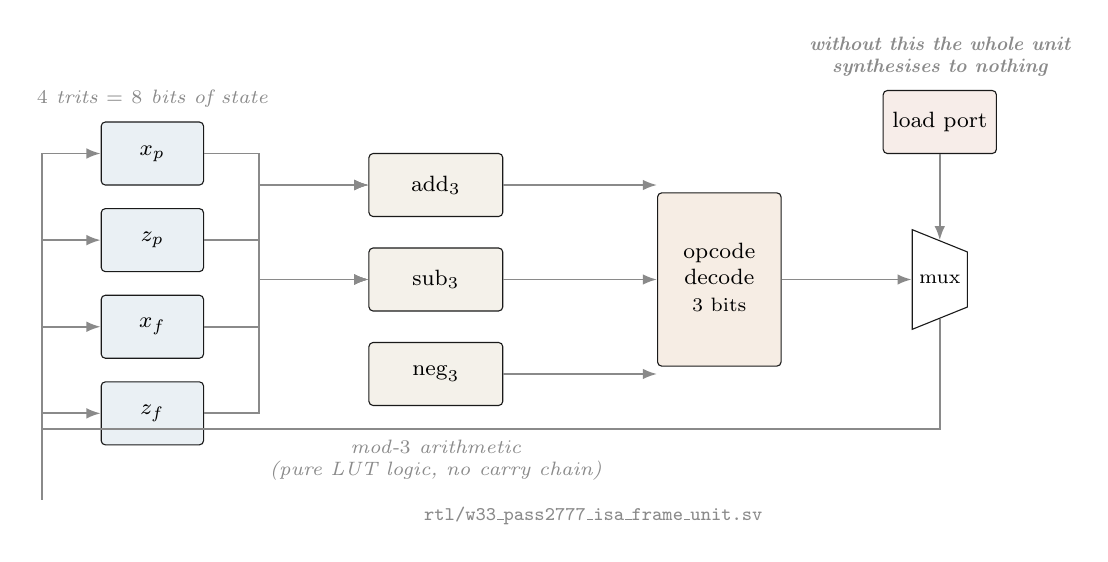
\begin{tikzpicture}[font=\footnotesize,>={Latex[length=2.2mm]},
  reg/.style={draw=ink,fill=specbg,minimum width=13mm,minimum height=8mm,rounded corners=1.5pt},
  alu/.style={draw=ink,fill=plainbg,minimum width=17mm,minimum height=8mm,rounded corners=1.5pt},
  mux/.style={draw=ink,fill=white,trapezium,trapezium angle=68,minimum width=9mm,
              minimum height=7mm,shape border rotate=270,inner sep=1pt},
  w/.style={-{Latex[length=1.8mm]},draw=rule,line width=0.7pt}]

  % registers
  \node[reg] (xp) at (0,3.0)  {$x_p$};
  \node[reg] (zp) at (0,1.9)  {$z_p$};
  \node[reg] (xf) at (0,0.8)  {$x_f$};
  \node[reg] (zf) at (0,-0.3) {$z_f$};
  \node[font=\scriptsize\itshape,text=rule,above=0.5mm of xp] {$4$ trits $=$ $8$ bits of state};

  % f3 units
  \node[alu] (a1) at (3.6,2.6) {$\mathrm{add}_3$};
  \node[alu] (a2) at (3.6,1.4) {$\mathrm{sub}_3$};
  \node[alu] (a3) at (3.6,0.2) {$\mathrm{neg}_3$};
  \node[font=\scriptsize\itshape,text=rule,align=center] at (3.6,-0.9)
    {mod-$3$ arithmetic\\(pure LUT logic, no carry chain)};

  % opcode decode
  \node[alu,minimum height=22mm,minimum width=15mm,fill=future!12] (dec) at (7.2,1.4)
    {\begin{tabular}{c}opcode\\decode\\\scriptsize $3$ bits\end{tabular}};

  % next-state mux
  \node[mux] (m) at (10.0,1.4) {};
  \node[font=\scriptsize] at (10.0,1.4) {mux};

  \node[reg,fill=warnbg] (ld) at (10.0,3.4) {load port};
  \node[font=\scriptsize\itshape,text=rule,align=center,above=0.5mm of ld]
    {\textbf{without this the whole unit}\\\textbf{synthesises to nothing}};

  \foreach \r in {xp,zp,xf,zf}{
    \draw[w] (\r.east) -- ++(0.7,0) |- (a1.west);
    \draw[w] (\r.east) -- ++(0.7,0) |- (a2.west);
  }
  \draw[w] (a1.east) -- (dec.west|-a1);
  \draw[w] (a2.east) -- (dec.west|-a2);
  \draw[w] (a3.east) -- (dec.west|-a3);
  \draw[w] (dec.east) -- (m.west);
  \draw[w] (ld.south) -- (m.north);
  \draw[w] (m.south) |- ++(0,-1.4) -| (-1.4,-1.4) |- (xp.west);
  \draw[w] (-1.4,-1.4) |- (zp.west);
  \draw[w] (-1.4,-1.4) |- (xf.west);
  \draw[w] (-1.4,-1.4) |- (zf.west);

  \node[font=\scriptsize,text=rule] at (5.6,-1.6)
    {\cmd{rtl/w33\_pass2777\_isa\_frame\_unit.sv}};
\end{tikzpicture}
\end{center}

\subsection{The measured cell budget}\label{sec:budget}

\begin{plain}
Below is what the machine actually costs, measured by running the industry-standard
open-source tools --- Yosys to translate the design into logic gates, nextpnr to place
those gates on a real chip --- targeting a Lattice iCE40 UP5K, a chip you can buy on a
breakout board for about \$25.

The entire arithmetic core of this computer is \emph{seventy-two} logic cells, out of
$5{,}280$ available. It uses $1.4\%$ of a \$25 chip.
\end{plain}

\begin{spec}[Measured; iCE40 UP5K SG48, Yosys 0.67 $+$ nextpnr]
\begin{center}\small
\begin{tabular}{@{}lrrl@{}}
\toprule
\textbf{Build} & \textbf{Logic cells} & \textbf{$F_{\max}$ (MHz)} & \textbf{Contains}\\
\midrule
$F$ only                 & 16 & 230.84 & one Fourier gate \\
$F_p + F_f$              & 19 & 230.84 & both Fourier gates \\
$F$ and $S$ (4 opcodes)  & 40 &  86.60 & the single-qutrit Cliffords \\
$\mathrm{CX}$ only       & 33 &  72.40 & the entangler, both directions \\
$\sigma^5{=}Z$ only      & 20 & 144.07 & the translation \\
all Clifford, no $Z$     & 65 &  60.80 & \textcolor{bad}{cannot leave the origin} \\
\textbf{full frame unit} & \textbf{72} & \textbf{60.80} & \textcolor{good}{the machine} \\
\midrule
\multicolumn{4}{@{}l}{\itshape For comparison, elsewhere in the design:}\\
$\mathrm{CX}$, bare loadable        &  23 & 72.40 & \cmd{w33\_pass2752\_cx\_loadable\_frame.sv}\\
$36$-lane mixer, serial            & 4048 & 19.65 & \cmd{w33\_pass2612\_serial\_mixer.sv}\\
$36$-lane mixer, parallel          & \multicolumn{2}{l}{13{,}965 LUT4 $+$ 799 carry} &
    \textcolor{bad}{does not fit any iCE40}\\
\bottomrule
\end{tabular}
\end{center}
\end{spec}

\begin{plain}
The last two rows are worth a moment. The ``mixer'' is the part that combines $36$
signals at once. Built the obvious way --- all $36$ lanes in parallel --- it needs
about $14{,}000$ logic cells, nearly twice what the largest chip in this family has. Built
serially, one lane at a time, it needs $4{,}048$: about a third of the area, at
$1/36$ of the speed. That is the kind of trade a blueprint exists to make explicit.
\end{plain}

\begin{gotwrong}
\textbf{Every cell count in this project before Pass 2753 was wrong, and the reason is
instructive.} We reported $13$ cells for $F$ and $S$, $8$ for $\mathrm{CX}$, $42$ for the
ISA. Those modules had no load port. By the reachability theorem of \S\ref{sec:isa}, a
register driven only by Clifford opcodes can never leave $(0,0,0,0)$ --- so the synthesis
tool \emph{proved the state was constant and deleted six of the eight flip-flops}. We were
measuring the area of nothing.

\medskip\noindent
Two independent teams shipped this same defect within four hours of each other. Both had
\emph{exhaustive} testbenches --- one covered all $81^2$ pairs of frames --- and both
passed, because the testbenches drove the \emph{combinational} logic and never
instantiated the sequential wrapper.

\medskip\noindent
\textbf{Simulation cannot detect this class of defect at all.} A module that folds to a
constant still simulates correctly. It just does nothing. Only a synthesis frontend asks
whether the state can move.

\medskip\noindent
One figure survived unchanged: $\sigma^5=Z$ was reported at $21$ cells and re-measures at
$20$. It was always real --- because it is the one instruction that is not linear, and so
the one instruction that could always move the state. The theory predicted exactly which
number would survive.
\end{gotwrong}

% =====================================================================================
\section{The physical layer}
% =====================================================================================

\begin{plain}
Everything above is logic --- it would work on any hardware that can implement the eight
operations. This section is about doing it with light, which is the intended
implementation, and about what has already been demonstrated in a laboratory as opposed
to designed on paper.

A single photon carries several independent properties. Two of them are useful here:
\emph{when} it arrives (its time bin) and \emph{what colour} it is (its frequency bin).
Chop time into three slots and colour into three bands, and one photon carries two
qutrits --- the ``past'' and ``future'' registers of \S\ref{sec:physics}.
\end{plain}

\begin{center}
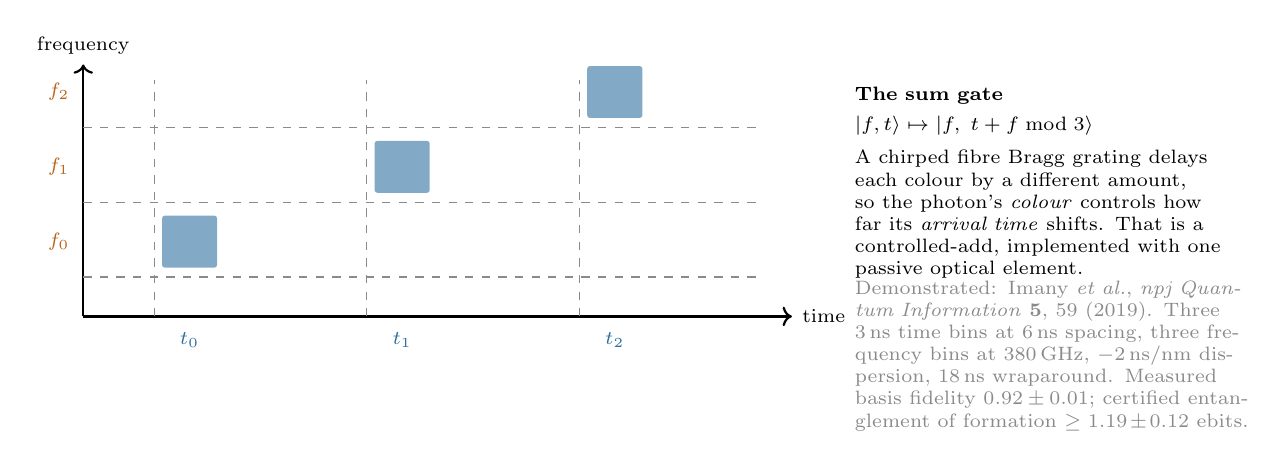
\begin{tikzpicture}[font=\footnotesize]
  \draw[->,line width=0.8pt] (0,0) -- (9.0,0) node[right,font=\scriptsize] {time};
  \draw[->,line width=0.8pt] (0,0) -- (0,3.2) node[above,font=\scriptsize] {frequency};
  \foreach \i in {0,1,2}{
    \draw[dashed,draw=rule] (0,\i*0.95+0.5) -- (8.6,\i*0.95+0.5);
    \draw[dashed,draw=rule] (\i*2.7+0.9,0) -- (\i*2.7+0.9,3.0);
  }
  \foreach \i in {0,1,2}{
    \node[font=\scriptsize,text=future,left] at (-0.05,\i*0.95+0.95) {$f_\i$};
    \node[font=\scriptsize,text=past,below] at (\i*2.7+1.35,-0.08) {$t_\i$};
  }
  \foreach \i in {0,1,2}{
    \fill[past!60,rounded corners=1pt]
      (\i*2.7+1.0,\i*0.95+0.62) rectangle (\i*2.7+1.7,\i*0.95+1.28);
  }
  \node[align=left,text width=5.0cm,font=\scriptsize] at (12.3,1.7)
   {\textbf{The \textsc{sum} gate}\\[3pt]
    $\ket{f,t}\mapsto\ket{f,\;t+f \bmod 3}$\\[4pt]
    A chirped fibre Bragg grating delays each colour by a different amount, so the
    photon's \emph{colour} controls how far its \emph{arrival time} shifts. That is a
    controlled-add, implemented with one passive optical element.};
  \node[align=left,text width=5.0cm,font=\scriptsize,text=rule] at (12.3,-0.5)
   {Demonstrated: Imany \emph{et al.}, \emph{npj Quantum Information} \textbf{5}, 59
    (2019). Three $3$\,ns time bins at $6$\,ns spacing, three frequency bins at
    $380$\,GHz, $-2$\,ns/nm dispersion, $18$\,ns wraparound. Measured basis fidelity
    $0.92\pm0.01$; certified entanglement of formation $\ge 1.19\pm0.12$ ebits.};
\end{tikzpicture}
\end{center}

\begin{spec}[Evidence boundary --- what is measured and what is not]
\textbf{Measured in a laboratory:} the deterministic single-photon qutrit \textsc{sum}
gate, at fidelity $0.92\pm0.01$, with the entangled output certified.

\smallskip\noindent
\textbf{Proved exactly:} the group theory, the geometry, the class atlas, the ISA
semantics, the reachability, the synthesis and placement figures.

\smallskip\noindent
\textbf{Neither, and stated as such:} source efficiency, insertion-loss engineering,
fault-tolerance thresholds, and the magic-state injection route. The $M_{36}$ resources
are typed \cmd{M36\_Q4\_RAW} in the controller and injection is \emph{refused} in RTL
until a proved ququart protocol supplies a validity assertion. That refusal is a design
feature: it makes the gap impossible to paper over.
\end{spec}

% =====================================================================================
\section{Why the exponent nine}
% =====================================================================================

\begin{plain}
A small but pretty result that shows how tightly the layers fit.

To tell which operation the machine just performed, you measure a quantity and look it up
in a table. The obvious quantity --- the ``trace'' --- has a flaw: it changes if the whole
state picks up an irrelevant overall phase, which physically means nothing. The fix used
in this project is to raise the trace to the \emph{ninth} power and divide by a
determinant. The ninth power was found empirically. Where does nine come from?
\end{plain}

\begin{spec}[Derived, Pass 2779]
For a $d$-dimensional representation, under $U\mapsto\lambda U$ we have
$\mathrm{Tr}(U^k)^e\mapsto\lambda^{ke}\,\mathrm{Tr}(U^k)^e$ and
$\det(U^k)\mapsto\lambda^{kd}\det(U^k)$, so
\[
  \Theta_k(g)=\frac{\mathrm{Tr}(U_g^k)^e}{\det(U_g^k)}
\]
is phase-invariant for all $\lambda$ \emph{exactly} when $e=d$. Here $d=9$, the dimension
of the two-qutrit state space --- which by \S\ref{sec:physics} is
$\dim\mathrm{End}(\mathbb{C}^3)$. Verified numerically: $e\in\{3,8,10\}$ fail, $e=9$ holds.

\smallskip\noindent
If the phase ambiguity were a \emph{finite} group $\mu_m$ one could use any
$e\equiv 9\pmod m$, possibly smaller. We computed the scalar subgroup of the generated
matrix group by collision sampling and it is $\mu_{12}$. Since $9\not\equiv 0\pmod{12}$,
the determinant is genuinely required, and $9$ is the \emph{smallest} exponent that
works: the sensor is minimal.
\end{spec}

\headline{$\mu_{12}=\mu_4\times\mu_3$. The $\mu_3$ is $\omega$, the qutrit alphabet.
The $\mu_4$ is the quadratic Gauss sum $\sum_j\omega^{j^2}=i\sqrt3$, which is
\emph{imaginary} precisely because $3\equiv 3 \pmod 4$ --- the same congruence that makes
time reversal a physical rather than a gauge symmetry.}

\begin{plain}
That last box is the kind of thing that makes this project worth doing. A practical
question --- ``why is the exponent nine in the measurement circuit?'' --- turns out to
have the same answer as an abstract one --- ``why does this geometry distinguish past
from future?''. Both are the statement that $-1$ is not a perfect square when you count
modulo $3$.
\end{plain}

\subsection{And for wider registers, it is usually three}

\begin{spec}[Pass 2791]
The phase group is not an artefact of the two-qutrit case. At $n=1$ the Clifford group is
small enough to enumerate exactly rather than sample:
\[
  |\langle F,S,X\rangle| = 2592 = \underbrace{12}_{\mu_{12}}\times
  \underbrace{216}_{|\mathrm{ASp}(2,3)|}\quad\text{--- consistent, so }\mu_{12}\text{ again.}
\]
For $n$ qutrits $d=3^n$, so the minimal exponent is the least $e\equiv 3^n \pmod{12}$, and
$3^n \bmod 12$ cycles $3,9,3,9,\dots$:
\[
\begin{array}{c|cccc}
n & 1 & 2 & 3 & 4\\\hline
d=3^n & 3 & 9 & 27 & 81\\
\text{minimal }e & \mathbf{3} & 9 & \mathbf{3} & 9
\end{array}
\]
Verified directly on $3\times3$ unitaries: $e=3$ is phase-invariant, $e\in\{2,4,9\}$ is not.
\end{spec}

\headline{Odd register widths need only a \emph{cube} of the trace, not a ninth power ---
a strictly cheaper measurement, alternating with width.}

% =====================================================================================
\section{The magic states, and the one thing the machine cannot yet do}\label{sec:magic}
% =====================================================================================

\begin{plain}
Everything described so far is, in a precise technical sense, \emph{not enough}. The
eight opcodes generate a large and useful group, but a machine restricted to those
operations can be simulated efficiently by an ordinary computer. To get a genuine quantum
advantage you need one more ingredient, traditionally supplied as a special prepared
state called a \emph{magic state}.

The substrate hands us $36$ candidates for free --- $36$ special directions in the
four-dimensional space, called the Witting rays. The open question, and the single
largest gap in this blueprint, is whether those $36$ can be \emph{purified}: whether many
noisy copies can be distilled into one clean one. Without that, the machine is a very
elegant classical simulator.
\end{plain}

\subsection{All thirty-six look identical from the inside}

% The optional argument is braced: an unbraced "]" inside $\mathbb{Z}[\omega]$ closes
% the optional argument early and LaTeX reports "Extra }, or forgotten $".
\begin{spec}[{Exact integer arithmetic in $\mathbb{Z}[\omega]$, Pass 2790}]
Only two overlap values occur among the $36$ rays:
\[
  |\langle i|j\rangle|^2 \in \{\,0,\ \tfrac13\,\},
\]
and every ray has the \emph{same} profile: $11$ orthogonal partners and $24$ partners at
overlap $1/3$. There is exactly one Gram profile among all $36$.

\smallskip\noindent
(The orthogonality graph is $11$-regular on $36$ vertices but \emph{not} strongly
regular: $\lambda\in\{1,2\}$, $\mu\in\{3,4\}$. Recorded because the near-miss invites a
false claim.)
\end{spec}

\begin{plain}
So no symmetry of the machine can tell one ray from another by looking at how they sit
relative to each other. If the rays differ at all, they differ only in how they sit
relative to the \emph{ordinary} states --- an external comparison, not an internal one.
\end{plain}

\subsection{And from the outside, they fall into exactly three grades}

\begin{spec}[$60$ two-qubit stabilizer states, $F_{\mathrm{stab}}=\max_s|\langle s|\psi\rangle|^2$]
\begin{center}
\begin{tabular}{@{}rlrl@{}}
\toprule
$F_{\mathrm{stab}}$ & closed form & rays & grade\\
\midrule
$0.750000$ & $9/12$              & \textbf{4}  & shallow\\
$0.705342$ & $(5+2\sqrt3)/12$    & \textbf{24} & mid\\
$0.622008$ & $(4+2\sqrt3)/12$    & \textbf{8}  & deep\\
\bottomrule
\end{tabular}
\end{center}
Stabilizer fidelity is a Clifford invariant, so the $8+24+4$ grading is genuine and not
an artefact of the chosen basis.
\end{spec}

\begin{spec}[All three noise thresholds are one formula]
For $\rho_p=(1-p)|m\rangle\!\langle m|+p\,I/4$ the target overlap is $1-3p/4$, so the
witness certifies non-stabilizerness exactly while $1-3p/4>F_{\mathrm{stab}}$:
\[
  \boxed{\;p \;<\; \tfrac{4}{3}\bigl(1-F_{\mathrm{stab}}\bigr)\;}
\]
\[
\begin{array}{lll}
\text{shallow} & 0.333333333333 & =\ 1/3\\
\text{mid}     & 0.392877598318 & =\ (7-2\sqrt3)/9\\
\text{deep}    & 0.503988709429 & =\ (8-2\sqrt3)/9
\end{array}
\]
Three separately-published thresholds, one formula, agreement to $10^{-12}$.
\end{spec}

\headline{The distillation search needs \emph{three} representatives, not thirty-six.
A Clifford-invariant protocol cannot distinguish rays within a grade.}

\begin{plain}
That is the practical payoff. The known result in this area is a \emph{no-go}: an
exhaustive search over $5{,}355$ small stabilizer codes and $21{,}420$ branches found no
two-copy protocol that improves fidelity anywhere it applies. The natural next move is to
search bigger protocols, and that search is expensive. Knowing there are only three
inequivalent starting materials shrinks it by a factor of twelve before it begins.
\end{plain}

\begin{spec}[Evidence boundary, stated as bluntly as possible]
No distillation protocol for $M_{36}$ is known. The controller types the resource
\cmd{M36\_Q4\_RAW} and \emph{refuses} injection in RTL until a proved protocol asserts
validity. \textbf{Until that assertion exists, this machine is not universal.} Everything
else in this blueprint is built or proved; this is not.
\end{spec}

% =====================================================================================
\section{The network}\label{sec:network}
% =====================================================================================

\subsection{Fractal scaling}

\begin{plain}
The machine is designed to be copied. A node contains $40$ sub-nodes; each sub-node
contains $40$ of its own; and so on. The network of machines has the same shape as the
inside of one machine --- which means one routing scheme, one addressing scheme, and one
error model serve every scale at once.
\end{plain}

\begin{center}
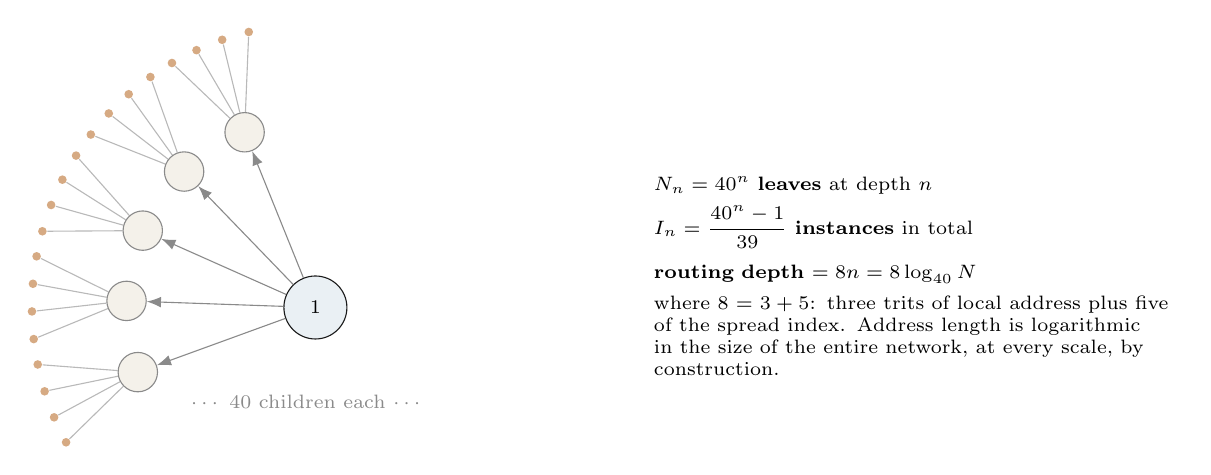
\begin{tikzpicture}[font=\scriptsize,>={Latex[length=1.8mm]},
  n0/.style={circle,draw=ink,fill=specbg,minimum size=8mm},
  n1/.style={circle,draw=rule,fill=plainbg,minimum size=5mm},
  n2/.style={circle,fill=future!55,inner sep=1.1pt}]
  \node[n0] (r) at (0,0) {$1$};
  \foreach \i [count=\k from 0] in {1,...,5}{
     \pgfmathsetmacro\ang{200-\k*22}
     \node[n1] (a\i) at (\ang:2.4) {};
     \draw[->,draw=rule] (r) -- (a\i);
     \foreach \j in {1,...,4}{
        \pgfmathsetmacro\bng{\ang-14+\j*5.6}
        \node[n2] (b\i\j) at (\bng:3.6) {};
        \draw[draw=rule,opacity=0.6] (a\i) -- (b\i\j);
     }
  }
  \node[font=\scriptsize,text=rule] at (-0.1,-1.2) {$\cdots$ $40$ children each $\cdots$};
  \node[align=left,text width=6.6cm] at (7.6,0.4)
   {\textbf{$N_n = 40^n$ leaves} at depth $n$\\[3pt]
    \textbf{$I_n = \dfrac{40^n-1}{39}$ instances} in total\\[5pt]
    \textbf{routing depth $= 8n = 8\log_{40}N$}\\[3pt]
    where $8 = 3+5$: three trits of local address plus five of the
    spread index. Address length is logarithmic in the size of the entire
    network, at every scale, by construction.};
\end{tikzpicture}
\end{center}

\subsection{Every bit string is a legal address}

\begin{spec}
The routing code has orbit sizes $162+162+324+648=1296$ on compass pairs, giving
codeword lengths $3,3,2,1$ and
\[
  2^{-3}+2^{-3}+2^{-2}+2^{-1} \;=\; 1 \quad\text{exactly (Kraft equality).}
\]
The prefix code is $\{110,111,10,0\}$ with expected length $7/4$. Because Kraft holds
with \emph{equality}, the decision tree has no unused branch: $20{,}000$ random bit
strings were parsed with $0$ failures.
\end{spec}

\begin{center}
\begin{tikzpicture}[font=\scriptsize,level distance=11mm,
  every node/.style={circle,draw=ink,inner sep=1.2pt},
  level 1/.style={sibling distance=34mm},
  level 2/.style={sibling distance=17mm},
  level 3/.style={sibling distance=11mm}]
\node {}
  child {node[fill=good!35,label=below:{\texttt{0}}] {} edge from parent node[draw=none,left,xshift=1mm]{$0$}}
  child {node {}
    child {node[fill=good!35,label=below:{\texttt{10}}] {} edge from parent node[draw=none,left,xshift=1mm]{$0$}}
    child {node {}
      child {node[fill=good!35,label=below:{\texttt{110}}] {} edge from parent node[draw=none,left,xshift=1mm]{$0$}}
      child {node[fill=good!35,label=below:{\texttt{111}}] {} edge from parent node[draw=none,right,xshift=-1mm]{$1$}}
      edge from parent node[draw=none,right,xshift=-1mm]{$1$}}
    edge from parent node[draw=none,right,xshift=-1mm]{$1$}};
\end{tikzpicture}
\end{center}

\begin{plain}
Look at the tree: every branch ends in a valid address. Nothing dangles.

The engineering consequence is unusual and worth stating plainly. In a normal computer, a
corrupted instruction stream can produce an \emph{illegal instruction} --- a bit pattern
that means nothing, which the processor must detect and trap. Here that cannot happen. A
corrupted packet is always a legal packet addressed somewhere else. The fault model
therefore has no ``decode error'' term at all; it has only a ``wrong result'' term. That
simplifies the error correction enormously, and it is forced by the geometry rather than
designed in.
\end{plain}

\begin{gotwrong}
We wrote that ``the consequence nobody has stated'' was that every bit string is a valid
instruction stream. The project's own holonet manuscript says it at line 382 --- ``the
routing words fill a binary decision tree with \emph{no unused branch}'' --- with a
citation to McMillan. This was the first error in this project caught by an automated
guard rather than by a human noticing. The engineering consequence drawn on top (no
decode-error term in the fault model) is a step past the coding fact and appears to be
new; the completeness property itself is the manuscript's.
\end{gotwrong}

\subsection{Remote operations}

\begin{spec}
A \textsc{sum} gate between two \emph{separate} machines costs exactly:
\[
  \boxed{\text{one shared qutrit Bell pair} \;+\; \text{two classical trits}}
\]
Protocol: Alice applies reverse local \textsc{sum} into her half of the pair, measures,
sends trit $m$; Bob applies $X^{-m}F^2$, applies direct \textsc{sum} to his data, measures
in the Fourier basis, sends trit $n$; Alice records $Z^n$ in her Pauli frame. All nine
branches implement $\ket{x,y}\mapsto\ket{x,y+x}$; verified on all nine basis inputs, all
nine branches, and $32$ random superpositions. Total conditional success probability $1$.
\end{spec}

% =====================================================================================
\section{Verification: how we know}\label{sec:verification}
% =====================================================================================

\begin{plain}
This is the section a working engineer should read first, because it is the one that
determines whether any of the preceding numbers mean anything.

The short version: this project has repeatedly shipped results that were verified in the
direction that would confirm them and never in the direction that would break them. Every
tool below exists because that happened at least three times.
\end{plain}

\begin{center}
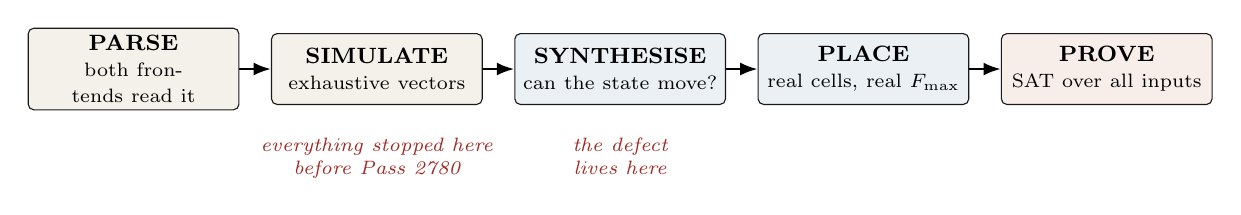
\begin{tikzpicture}[font=\footnotesize,>={Latex[length=2.2mm]},
  st/.style={draw=ink,rounded corners=2pt,minimum height=9mm,text width=25mm,align=center,
             inner sep=2.5pt}]
  \node[st,fill=plainbg] (p) {\textbf{PARSE}\\\scriptsize both frontends read it};
  \node[st,fill=plainbg,right=4mm of p] (s) {\textbf{SIMULATE}\\\scriptsize exhaustive vectors};
  \node[st,fill=specbg,right=4mm of s] (y) {\textbf{SYNTHESISE}\\\scriptsize can the state move?};
  \node[st,fill=specbg,right=4mm of y] (n) {\textbf{PLACE}\\\scriptsize real cells, real $F_{\max}$};
  \node[st,fill=warnbg,right=4mm of n] (f) {\textbf{PROVE}\\\scriptsize SAT over all inputs};
  \foreach \a/\b in {p/s,s/y,y/n,n/f}{\draw[->,line width=0.9pt] (\a) -- (\b);}
  \node[font=\scriptsize\itshape,text=bad,align=center,below=3mm of s]
    {everything stopped here\\before Pass 2780};
  \node[font=\scriptsize\itshape,text=bad,align=center,below=3mm of y]
    {the defect\\lives here};
\end{tikzpicture}
\end{center}

\begin{spec}[The five automated guards, each built from a measured failure]
\begin{center}\small
\scriptsize\begin{tabular}{@{}p{4.2cm}p{4.1cm}p{4.7cm}@{}}
\toprule
\textbf{Guard} & \textbf{Catches} & \textbf{Built because}\\
\midrule
\cmd{check\_rediscovery.py} &
  a staged file asserts a code parameter that exists elsewhere uncited &
  $21\%$ of $173$ files did this (census, Pass 328) \\
\cmd{check\_certificates.py} &
  a frozen certificate that cannot reproduce its own digest &
  one was unverifiable \emph{from birth} and passed every check while being so \\
\cmd{check\_novelty\_claims.py} &
  explicit novelty phrases whose tokens are in the encyclopedia &
  five claims in one session were overturned by files we had not read \\
\cmd{check\_implicit\_novelty.py} &
  \emph{emphasised} results carried by a source the file never cites &
  four of six failures never used a novelty phrase at all \\
\cmd{check\_rtl\_folds.py} &
  an output port tied to a literal after full optimisation &
  two independent teams shipped a module that synthesises to the identity \\
\bottomrule
\end{tabular}
\end{center}
All five \textbf{warn and never block}. A collision is a candidate for reading, not a
verdict, and a blocking hook trains people to pass \cmd{-{}-no-verify}.
\end{spec}

\begin{gotwrong}
\textbf{The guards themselves needed calibration, and the calibration is the work.}
\cmd{check\_implicit\_novelty.py} went through four measured versions:
\begin{center}\small
\begin{tabular}{@{}rll@{}}
\toprule
\textbf{Flagged} & \textbf{Version} & \textbf{What the noise turned out to be}\\
\midrule
$9/122$  & presence of any token & all nine were \emph{pass numbers in titles}\\
$0/122$  & $+$ skip files citing ``Prior art'' &
   \textcolor{bad}{vacuous} --- every file has that section\\
$51/122$ & $+$ cite the \emph{right} source per token & \texttt{W(3,3)} $21\times$: the repo's own subject\\
$27/122$ & $+$ rarity and non-round integers & what ships\\
\bottomrule
\end{tabular}
\end{center}
The second row is the instructive one: \textbf{a guard that passes everything looks
exactly like a guard that finds nothing wrong.} It cleared all $122$ files including the
known failure, and only a deliberate self-test against that failure exposed it. Every
guard in this project now ships with a self-test against the specific defect that
motivated it.

\medskip\noindent
\cmd{check\_rtl\_folds.py} had the same disease on its first run: it reported a clean
sweep because the WSL mount is \cmd{/mnt/c} while Python resolves the drive as
\cmd{C:}, so every directory change failed silently and no netlist was ever produced. It
now reports \textsc{not synthesized} explicitly rather than treating a missing netlist as
a pass.
\end{gotwrong}

% =====================================================================================
\section{The complete ledger}
% =====================================================================================

\begin{plain}
Everything this blueprint asserts, with how it is known. If a row says
``proved'' there is a machine-checkable artifact; if it says ``measured'' there is a tool
output; if it says ``published'' someone else did it and we cite them.
\end{plain}

{\small
\begin{center}
\begin{tabular}{@{}p{8.6cm}p{2.5cm}p{4.0cm}@{}}
\toprule
\textbf{Claim} & \textbf{Status} & \textbf{Artifact}\\
\midrule
$W(3,3)$ has $\mathrm{SRG}(40,12,2,4)$ collinearity graph & classical & literature\\
$40=(3^4-1)/2$ from one self-entangled qutrit & proved & Pass 2724\\
The one-qutrit thesis itself & \textbf{prior art} & \cmd{index.html} MCLXVII\\
Outer involution $=$ transpose $=$ time reversal & proved at $q{=}3$ & Pass 2732\\
Time reversal outer $\iff q\equiv 3\pmod 4$ & proved & Pass 2750\\
Transpose \emph{constructed} and checked at $q\le 23$ & proved & Pass 2792, 8 primes\\
Anti-symplectic $T$, $T^\top JT=-J$; class action $10$ pairs $+$ $14$ fixed
   & proved & parallel track, Pass 2762\\
Six Clifford opcodes reach $1$ frame of $81$ & proved & Pass 2774 (BFS)\\
Full ISA reaches all $81$ & proved & Pass 2774\\
Clifford opcodes generate $\mathrm{Sp}(4,3)$, order $51{,}840$ & proved & Pass 2778\\
Full ISA generates $\mathrm{ASp}(4,3)$, order $4{,}199{,}040$ & proved & Pass 2778\\
One translation generator suffices (orbit $=80$) & proved & Pass 2778\\
Minimal Clifford subset has size $3$; sizes $1,2$ give none & proved & Pass 2789, 6 triples\\
Frame ISA fits a \textbf{two-bit} opcode field & follows & Pass 2789\\
Sensor exponent $9=\dim$; phase group $\mu_{12}$; $9$ minimal & proved & Pass 2779\\
$\mu_4$ factor $=$ imaginary Gauss sum & proved & Pass 2779\\
$\mu_{12}$ at $n{=}1$ by exact enumeration ($2592=12\cdot216$) & proved & Pass 2791\\
Minimal exponent $=3^n\bmod 12$: $3$ odd, $9$ even & derived & Pass 2791\\
$36$ rays share one Gram profile ($11$ orth., $24$ at $1/3$) & proved & Pass 2790, $\mathbb{Z}[\omega]$\\
$8{+}24{+}4$ is the stabilizer-fidelity spectrum & proved & Pass 2790, 60 stab.\ states\\
All three witness thresholds $=\frac43(1-F_{\mathrm{stab}})$ & derived & Pass 2790, $10^{-12}$\\
$M_{36}$ two-copy no-go, $5355$ codes $\times$ $4$ syndromes & \textbf{prior art} & parallel track, Pass 2784\\
Frame unit: $72$ LC, $60.80$\,MHz & \textbf{measured} & \S\ref{sec:budget}\\
Loadable CX: $23$ LC, $72.40$\,MHz, $\mathrm{CX}^3{=}I$ & measured $+$ proved &
   $5265$ vars / $14005$ clauses\\
Parallel $36$-mixer: $13{,}965$ LUT4, does not fit & measured & Pass 2773\\
Signed mixer correct on impulse class & proved & $1{,}097{,}152$ vars\\
Kraft equality; $0$ parse failures in $20{,}000$ & proved $+$ measured & Pass 2682\\
Photonic qutrit \textsc{sum}, fidelity $0.92\pm0.01$ & \textbf{published} &
   Imany \emph{et al.}\ 2019\\
Remote \textsc{sum}: $1$ Bell pair $+$ $2$ trits & proved & parallel track, Pass 2771\\
\midrule
$M_{36}$ magic-state injection threshold & \textcolor{bad}{OPEN} & refused in RTL\\
Fault-tolerance threshold end to end & \textcolor{bad}{OPEN} & --- \\
Physical power in watts & \textcolor{bad}{OPEN} & activity proxy only\\
\bottomrule
\end{tabular}
\end{center}}

% =====================================================================================
\section{Reproducing everything in this document}
% =====================================================================================

\begin{spec}[Commands, in order]
\begin{quote}\ttfamily\small
\# reachability and the group\\
py -3 analysis/w33\_pass2774\_isa\_frame\_reachability.py\\
py -3 analysis/w33\_pass2778\_2779\_affine\_group\_and\_sensor\_exponent.py\\[4pt]
\# the cell budget (needs yosys + nextpnr-ice40)\\
yosys -p "read\_verilog -sv rtl/w33\_pass2777\_isa\_frame\_unit.sv; \textbackslash\\
\hspace*{1em}chparam -set EN 63 w33\_isa\_frame\_unit; \textbackslash\\
\hspace*{1em}synth\_ice40 -top w33\_isa\_frame\_unit -json u.json"\\
nextpnr-ice40 -{}-up5k -{}-package sg48 -{}-json u.json -{}-asc u.asc -{}-freq 50\\[4pt]
\# the formal proofs\\
yosys -p "read\_verilog -sv -formal rtl/w33\_pass2752\_cx\_loadable\_frame.sv; \textbackslash\\
\hspace*{1em}prep -top w33\_cx\_loadable\_formal -flatten; async2sync; \textbackslash\\
\hspace*{1em}chformal -lower; sat -seq 8 -prove-asserts -verify"\\[4pt]
\# the guards\\
py -3 scripts/check\_rtl\_folds.py\\
py -3 scripts/check\_implicit\_novelty.py\\
py -3 scripts/check\_novelty\_claims.py\\[4pt]
\# this document\\
tectonic holonet\_machine\_blueprint.tex
\end{quote}
\end{spec}

% =====================================================================================
\section{What is not built}
% =====================================================================================

\begin{plain}
A blueprint that lists only what works is advertising. Here is the honest remainder.
\end{plain}

\begin{enumerate}[leftmargin=*,itemsep=3pt]
\item \textbf{Two of the eight opcodes are not frame operations and are not built as
      such.} $D_{12}$-mirror is a transport operation in a dihedral group; $M_{36}$-magic
      is deliberately a \emph{handshake} to an external state-preparation block, and the
      controller \emph{refuses} injection until a proved protocol asserts validity. No
      non-Clifford unitary is invented in RTL, because inventing one would conceal the
      real gap.
\item \textbf{The magic-state route is the universality gap.} The substrate identifies
      $36$ distinguished Witting rays and computes exact non-stabilizer witness
      boundaries for them. It does \emph{not} supply a distillation protocol; the
      published qutrit protocols act on a different space (ququart versus qutrit) and do
      not transfer.
\item \textbf{No physical power figure exists.} The switching census gives about $1.622$
      output transitions per operation. That is a technology-independent activity proxy.
      Watts require the placed netlist, a capacitance model, voltage, clock and a
      representative workload.
\item \textbf{(Closed at Pass 2792.)} The transpose construction was previously
      verified at $q=3$ only. It is now built and checked over $\mathbb{F}_q$ at
      $q=3,5,7,11,13,17,19,23$: $T^2=I$ and $T^\top JT=-J$ hold at every one, and the
      congruence law holds at every one. Left in this list, struck through, because a
      blueprint should show which gaps closed and when.
\item \textbf{One original module is unparseable} ---
      \cmd{rtl/w33\_spread\_mixer36.sv}, rejected by both frontends. It now carries a
      deprecation banner naming its replacement and quoting both errors; the bytes are
      kept as the historical record, since it compiles nowhere and deleting another
      track's file is not ours to do.
\end{enumerate}

\vspace{6mm}
\begin{center}
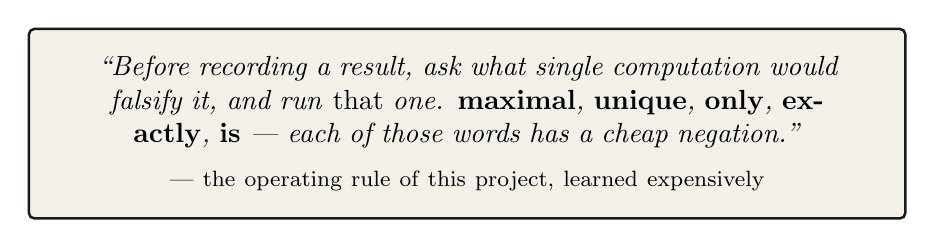
\begin{tikzpicture}
 \node[draw=ink,line width=0.9pt,rounded corners=2pt,inner sep=10pt,
       text width=0.86\linewidth,align=center,fill=plainbg]
 {\itshape ``Before recording a result, ask what single computation would falsify it,
   and run \emph{that} one. \textnormal{\textbf{maximal}}, \textnormal{\textbf{unique}},
   \textnormal{\textbf{only}}, \textnormal{\textbf{exactly}}, \textnormal{\textbf{is}} ---
   each of those words has a cheap negation.''\\[4pt]
   \normalfont\footnotesize --- the operating rule of this project, learned expensively}
 ;
\end{tikzpicture}
\end{center}

\end{document}
